% https://github.com/martinhelso/MathDept


\documentclass[UKenglish,8pt,aspectratio=1610]{beamer}


\usetheme[NoLogo]{MathDept}

\usepackage{varwidth}
\usepackage[utf8]{inputenx} % For æ, ø, å
\usepackage{babel}          % Automatic translations
\usepackage{csquotes}       % Quotation marks
\usepackage{microtype}      % Improved typography
\usepackage{amssymb}        % Mathematical symbols
\usepackage{mathtools}      % Mathematical symbols
\usepackage[absolute, overlay]{textpos} % Arbitrary placement
\setlength{\TPHorizModule}{\paperwidth} % Textpos units
\setlength{\TPVertModule}{\paperheight} % Textpos units
\usepackage{tikz}
\usetikzlibrary{overlay-beamer-styles}  % Overlay effects for TikZ
\usepackage{dsfont}
\usepackage{fontawesome5}
\author{Thomas Aussaguès}
\title{Project 2}
\subtitle{Estimation theory}
\usepackage{siunitx}
\usepackage{graphics}
\graphicspath{{../jupyter/images/}}	

\usepackage{color}
\definecolor{darkred}{rgb}{0.6,0.0,0.0}
\definecolor{darkgreen}{rgb}{0,0.50,0}
\definecolor{lightblue}{rgb}{0.0,0.42,0.91}
\definecolor{orange}{rgb}{0.99,0.48,0.13}
\definecolor{grass}{rgb}{0.18,0.80,0.18}
\definecolor{pink}{rgb}{0.97,0.15,0.45}

% listings
\usepackage{listings}

% Python style for highlighting


\begin{document}




% General Setting of listings
\lstset{
	aboveskip=1em,
	breaklines=true,
	abovecaptionskip=-6pt,
	captionpos=b,
	escapeinside={\%*}{*)},
	frame=single,
	numbers=left,
	numbersep=15pt,
	numberstyle=\tiny,
}
% 0. Basic Color Theme
\lstdefinestyle{colored}{ %
	basicstyle=\ttfamily,
	backgroundcolor=\color{gray},
	commentstyle=\color{green}\itshape,
	keywordstyle=\color{blue}\bfseries\itshape,
	stringstyle=\color{red},
}
% 1. General Python Keywords List
\lstdefinelanguage{PythonPlus}[]{Python}{
	morekeywords=[1]{,as,assert,nonlocal,with,yield,self,True,False,None,} % Python builtin
	morekeywords=[2]{,__init__,__add__,__mul__,__div__,__sub__,__call__,__getitem__,__setitem__,__eq__,__ne__,__nonzero__,__rmul__,__radd__,__repr__,__str__,__get__,__truediv__,__pow__,__name__,__future__,__all__,}, % magic methods
	morekeywords=[3]{,object,type,isinstance,copy,deepcopy,zip,enumerate,reversed,list,set,len,dict,tuple,range,xrange,append,execfile,real,imag,reduce,str,repr,}, % common functions
	morekeywords=[4]{,Exception,NameError,IndexError,SyntaxError,TypeError,ValueError,OverflowError,ZeroDivisionError,}, % errors
	morekeywords=[5]{,ode,fsolve,sqrt,exp,sin,cos,arctan,arctan2,arccos,pi, array,norm,solve,dot,arange,isscalar,max,sum,flatten,shape,reshape,find,any,all,plot,linspace,legend,quad,polyval,polyfit,hstack,concatenate,vstack,column_stack,empty,zeros,ones,rand,vander,grid,pcolor,eig,eigs,eigvals,svd,qr,tan,det,logspace,roll,min,mean,cumsum,cumprod,diff,vectorize,lstsq,cla,eye,xlabel,ylabel,squeeze,correlate,argmax,abs,np.}, % numpy / math
}
% 2. New Language based on Python
\lstdefinelanguage{PyBrIM}[]{PythonPlus}{
	emph={d,E,a,Fc28,Fy,Fu,D,des,supplier,Material,Rectangle,PyElmt},
}
% 3. Extended theme
\lstdefinestyle{colorEX}{
	basicstyle=\ttfamily,
	backgroundcolor=\color{gray!10},
	commentstyle=\color{darkgreen}\slshape,
	keywordstyle=\color{blue}\bfseries\itshape,
	keywordstyle=[2]\color{blue}\bfseries,
	keywordstyle=[3]\color{grass},
	keywordstyle=[4]\color{red},
	keywordstyle=[5]\color{orange}\bfseries,
	stringstyle=\color{darkred},
	emphstyle=\color{pink}\underbar,
}


\begin{frame}{Table of contents}
    \tableofcontents
\end{frame}

\section{Introduction}
\begin{frame}
\frametitle{Introduction}
	\begin{columns}
	\begin{column}{0.5\textwidth}
		\vspace{-10pt}
	\begin{figure}[h!]
		\begin{tikzpicture}
			\draw [fill=blue!30,rounded corners,blue!30] (0,0) rectangle (5,-3);
			\draw (1,0) node {$\bullet$};
			\draw (1,0) node [above ]{Sonar};
			\draw (4,-2) node [below] {Target};
			\draw (4,-2) node {\faFish};
			\draw [fill=brown!80,rounded corners,brown!80] (0,-2.5) rectangle (5,-3);
			\draw [red,<->,thick](1.1,-0.1)--(3.8,-1.8);
			\draw (2.45,-0.65) node {\textcolor{red}{$d$}};
			\draw (2.4,-2.75) node {Seafloor};
		\end{tikzpicture}
		\caption{Target detection and ranging}
	\end{figure}
	\end{column}
	\begin{column}{0.5\textwidth}
	\begin{itemize}
	\item \textcolor{red}{\textbf{Goal : estimate the distance between the sonar and the target $d$}}
	\item How can we estimate $d$ ? 
	\item By sending a pulse $s_{T_x}(t)$ and recording the pulse echo
	\item Using the delay $\tau_0$, we can acess $d$ 
	\begin{equation}
		d=\dfrac{c\tau_0}{2}
	\end{equation}
	\item But how to estimate the lag $\tau_0$ ? 
	\item \textcolor{red}{\textbf{Find the pulse start time in the echo}}
	\end{itemize}
	\end{column}
\end{columns} 

	\begin{columns}
	\begin{column}{0.5\textwidth}
		\vspace{-10pt}
		\begin{figure}[h!]
	\begin{figure}[h!]
	\centering
	\includegraphics[scale=0.4]{pulse.png}
	\caption{Sonar sent pulse}
\end{figure}
		\end{figure}
	\end{column}
	\begin{column}{0.5\textwidth}
		\vspace{-10pt}
	\begin{figure}[h!]
		\centering
		\includegraphics[scale=0.4]{sonar_data_1.png}
		\caption{Sonar recorded echo}
	\end{figure}
	\end{column}
\end{columns} 

\end{frame}

\section{Maximum likelihood estimator (MLE)}
\begin{frame}{Table of contents}
	\tableofcontents[currentsection]
\end{frame}
\begin{frame}
	\frametitle{MLE expression}
\begin{itemize}
	\item Discrete signal model : 
	\begin{equation}
		0\leq n\leq N-1,x[n]=\begin{cases}
			s[n-n_0]+w[n]&n_0\leq n\leq n_0 + M - 1\\
			w[n]&\textrm{otherwise}
		\end{cases}
	\end{equation} where $w[n]$ is some AWGN, $s[n]$ the pulse and $n_0 = \lfloor f_s\tau_0\rfloor$ with $f_s$ the sampling frequency
\item We assume that all samples are \textcolor{red}{\textbf{statistically independent}}\footnote{Or at least uncorrelated}
\item Likelihood function $\mathcal{L}\left(x[0],\dots,x[N-1],n_0\right)=\mathcal{L}(\mathbf{x},n_0)$
\item \textcolor{red}{\textbf{Goal : maximizing $\mathcal{L}(\mathbf{x},n_0)$ w.r.t. $n_0$}} 
\end{itemize}
	\begin{equation}
		\begin{aligned}
		\only<1-2>{\mathcal{L}(\mathbf{x},n_0)&=\prod_{n=0}^{n=n_0-1}\dfrac{1}{\sqrt{2\pi\sigma^2}}\exp\left(\dfrac{-x[n]^2}{2\sigma^2}\right)\times \prod_{n=n_0}^{n=n_0+M-1}\dfrac{1}{\sqrt{2\pi\sigma^2}}\exp\left(\dfrac{-(x[n]-s[n-n_0])^2}{2\sigma^2}\right)\\
		&\times \prod_{n=n_0+M}^{n=N-1}\dfrac{1}{\sqrt{2\pi\sigma^2}}\exp\left(\dfrac{-x[n]^2}{2\sigma^2}\right)\\}
		%%%%%%%%
		\only<2>{&=\dfrac{1}{\left(2\pi\sigma^2\right)^{N/2}}\prod_{n=0}^{n=n_0-1}\exp\left(\dfrac{-x[n]^2}{2\sigma^2}\right)\times\prod_{n=n_0}^{n=n_0+M-1}\exp\left(-\dfrac{x[n]^2-2x[n]s[n-n_0]+s[n-n_0]^2}{2\sigma^2}\right)\\
		&\times \prod_{n=n_0+M}^{n=N-1}\exp\left(\dfrac{-x[n]^2}{2\sigma^2}\right)}
		%%%%%%%%
		\only<3-4>{\mathcal{L}(\mathbf{x},n_0)&=\dfrac{1}{\left(2\pi\sigma^2\right)^{N/2}}\prod_{n=0}^{n=n_0-1}\exp\left(\dfrac{-x[n]^2}{2\sigma^2}\right)\times\prod_{n=n_0}^{n=n_0+M-1}\exp\left(-\dfrac{x[n]^2-2x[n]s[n-n_0]+s[n-n_0]^2}{2\sigma^2}\right)\\
		&\times \prod_{n=n_0+M}^{n=N-1}\exp\left(\dfrac{-x[n]^2}{2\sigma^2}\right)\\}
		%%%%%%%%
		\only<4-8>{&=\dfrac{1}{\left(2\pi\sigma^2\right)^{N/2}}\prod_{n=0}^{n=N-1}\exp\left(\dfrac{-x[n]^2}{2\sigma^2}\right)\times\prod_{n=n_0}^{n=n_0+M-1}\exp\left(\dfrac{x[n]s[n-n_0]}{\sigma^2}\right)\times \prod_{n=n_0}^{n=n_0+M-1}\exp\left(\dfrac{-s[n-n_0]^2}{2\sigma^2}\right)\\}
		%%%%%%%%
		&\only<5-8>{=\textcolor{blue}{\underbrace{\dfrac{1}{\left(2\pi\sigma^2\right)^{N/2}}\prod_{n=0}^{n=N-1}\exp\left(\dfrac{-x[n]^2}{2\sigma^2}\right)}_{\textrm{independent~of }~n_0}}}\only<6-8>{\times\textcolor{red}{\underbrace{\prod_{n=n_0}^{n=n_0+M-1}\exp\left(\dfrac{x[n]s[n-n_0]}{\sigma^2}\right)}_{J(n_0),~\textrm{to~maximize}}}}\only<7-8>{\times \textcolor{blue}{\underbrace{\prod_{n=n_0}^{n=n_0+M-1}\exp\left(\dfrac{-s[n-n_0]^2}{2\sigma^2}\right)}_{\textrm{independent~of }~n_0}}}
		\end{aligned}
	\end{equation}
\only<8>{\begin{itemize}
	\item So maximizing $\mathcal{L}(\mathbf{x},n_0)$ w.r.t. $n_0$ $\Longleftrightarrow$ maximizing the \textcolor{red}{\textbf{red term $J(n_0)$}} 
\end{itemize}}
\end{frame}

\begin{frame}
	\frametitle{MLE  expression 2}
	\begin{itemize}
		\item Since $s[n]$ is zero outside $\left[n_0,n_0+M-1\right]$, we can expand the product 
\end{itemize}
\begin{equation}
	\begin{aligned}
	J(n_0)&=\prod_{n=n_0}^{n=n_0+M-1}\exp\left(\dfrac{x[n]s[n-n_0]}{\sigma^2}\right)\only<2->{=\textcolor{red}{\prod_{n=0}^{n=N-1}}\exp\left(\dfrac{x[n]s[n-n_0]}{\sigma^2}\right)=\exp\left(\dfrac{1}{\sigma^2}\sum_{n=0}^{N-1}x[n]s[n-n_0]\right)}\\
	\only<4->{&=\exp\left(C_{xs}(n_0)\right)}
	\end{aligned}
\end{equation}
\only<3->{\begin{itemize}
	\only<3->{\item Assuming that we have jointly W.S.S. processes, we identify the cross-correlation $C_{xs}(n_0)=\displaystyle\sum_{n=0}^{N-1}x[n]s[n-n_0]$}
	\only<3->{\item We omit the conjugate here ($s[n-n_0]^\star$) }
	\only<4->{\item The exponential function is strictly increasing}
	\only<4->{\item \textcolor{red}{\textbf{Therefore, to maximize the likelihood, we must find $n_0$ maximizing the cross-correlation!}}}
\end{itemize}}
\end{frame}

\begin{frame}[fragile]
	\frametitle{\texttt{Python} implementation}
	\begin{figure}[h!]
	\begin{lstlisting}[language=PythonPlus,style=colorEX]
def generate_pulse(B,T_p,N_t,fs) :
	
	alpha = B/T_p
	time = np.arange(0,T_p+1/fs,1/fs)
	pulse = np.zeros((int(T_p*fs)),dtype='complex')
	pulse = np.exp(2*1j*np.pi*alpha*time**2/2)
	return pulse
	
def ml_time_delay_estimator(time_sequence,fs,c):
	
	# We generate a pulse
	pulse = generate_pulse(B,T_p,N_t,fs)
	# We compute the cross-corrleation between the generated pulse and 
	# the received signal (only for the first 1600 time samples, np.correlate compute cros-correlation only for positive lags)
	# We normalized the ouptut
	cross_correlation = np.correlate(time_sequence, pulse)[:1600]*1/1600 
	# We compute the index corresponding to the cross-correlation magnitude maximum 
	max_index = np.argmax(np.abs(cross_correlation))
	# Therefore, we can compute the correponding lag and distance
	# We must add t_0 to the lag as the sonar data starts at t_0
	lag = max_index/fs + t_0
	return lag
\end{lstlisting}
\centering
\caption{Python codes}
	\end{figure}
\end{frame}

\begin{frame}
	\frametitle{Time delay estimation}
		\begin{columns}
		\begin{column}{0.5\textwidth}
			\vspace{-25pt}
			\begin{figure}[h!]
				\includegraphics[scale=0.5]{normalized_mag_before_after_channel_1.png}
				\centering
				\caption{Sonar recorded echo and pulse compressed signal}
			\end{figure}
		\end{column}
		\begin{column}{0.5\textwidth}
		\begin{itemize}
			\item Both signals have been normalized
			\item One unique peak at approximately $0.017~\si{\milli\second}$
			\item At lag $0.017~\si{\milli\second}$, the pulse overlaps the echo
			\item Maximum cross-correlation
			\item Elsewhere, the pulse only partially overlaps the echo, so the cross-correlation $\rightarrow 0$
			\item Random noise and pulse are uncorrelated
			\item Moreover, the pulse is equal to 0 outside $[0,T_p]$, some samples ($x[n]\times 0$, zero-padding) are ignored in the cross-correlation !
			\item Higher SNR : the cross-correlation acts as a "noise filter"
		\end{itemize}
		\end{column}
	\end{columns} 
	
\end{frame}


\begin{frame}
	\frametitle{First results}
		\begin{columns}
		\begin{column}{0.5\textwidth}
			\vspace{-25pt}
			\begin{figure}[h!]
				\includegraphics[scale=0.5]{results.png}
				\centering
				\caption{Lag estimations, $f_s=40~\si{\kilo\hertz}$}
			\end{figure}
		\end{column}
		\begin{column}{0.5\textwidth}
		\begin{itemize}
			\item Lag estimations are increasing as function of the hydrophone
			\item 3 different domains
			\item Estimations are constant on these domains
		\end{itemize}
		\end{column}
	\end{columns} 
\end{frame}
\begin{frame}
	\frametitle{\textsc{NYQUIST-SHANNON} sampling theorem}
\begin{theorem}[\textsc{NYQUIST-SHANNON} sampling theorem]
If a continuous-variable signal is band-limited to frequencies below $f$, then it can be periodically sampled without loss of information so long as the sampling frequency $f_s\geq 2f$.
\end{theorem}
\begin{itemize}
	\item Sampling frequency $f_s=40~\si{\kilo\hertz}$
	\item What is the pulse maximum frequency ?
\end{itemize}
	\begin{columns}
	\begin{column}{0.5\textwidth}
	\only<2->{\begin{itemize}
		\item Pulse model
	\end{itemize}
\begin{equation}
	s_{T_x}(t)=\begin{cases}
		\exp\left(2j\pi\alpha\dfrac{t^2}{2}\right) & \rvert t\lvert < T_p/2\\
		0&\mathrm{elsewhere}
	\end{cases}
\end{equation}}
\only<3->{\begin{itemize}
\item Instantaneous frequency
\end{itemize}}
\only<4->{\begin{equation}
	\only<4->{f(t)=\dfrac{1}{2\pi}\dfrac{\mathrm{d}\phi(t)}{\mathrm{d}t}}\only<5->{=\dfrac{1}{2\pi}\dfrac{\mathrm{d}}{\mathrm{d}t}\left(2\pi\alpha\dfrac{t^2}{2}\right)=\alpha t}
\end{equation}} \only<4->{with $\phi$ the pulse phase}
\only<6->{\begin{itemize}
	\item Maximum frequency : when $t=T_p$
\end{itemize}
\begin{equation}
	f_{max}=\alpha T_p = \dfrac{B}{T_p}T_p=B=30~\si{\kilo\hertz}
\end{equation}
\begin{itemize}
	\item \textcolor{red}{\textbf{$f_s\ngeq 2f_{max}=2\times30~\si{\kilo\hertz}$ !}}
\end{itemize}}
	\end{column}
	\begin{column}{0.5\textwidth}
		\vspace{-25pt}
	\only<7->{\begin{figure}[h!]
		\includegraphics[scale=0.5]{pulse_spectrogram.png}
		\centering
		\caption{Pulse spectrogram}
	\end{figure}}
	\end{column}
\end{columns}
\end{frame}

\begin{frame}
\frametitle{Estimations using upsampled data}
\begin{itemize}
	\item Upsampling of a factor $n$ using MATLAB function \texttt{resample}
	\item Consequence : new sampling frequency $f_s'=nf_s$ (for both sequences)
	\item SHANNON theorem : \textcolor{green}{\faCheck} (at least for the pulse, AWGN has a higher frequency)
\end{itemize}

	\begin{columns}
	\begin{column}{0.5\textwidth}
	\vspace{-25pt}
	\begin{figure}[h!]
		\includegraphics[scale=0.5]{all_results.png}
		\centering
		\caption{Lag estimations, $f_s=40,120~\textrm{and}~240~\si{\kilo\hertz}$}
	\end{figure}
	\end{column}
	\begin{column}{0.5\textwidth}
	\begin{itemize}
	   %	\item We know that the fish is approximately at $12~\si{\meter}$ from the sonar
		%\item $\tau=\dfrac{2d}{c}=\dfrac{2\times 12}{1480}\approx 0.0162~\si{\second}$
		\item Upsampling factors $n=4$ and $n=8$ produced the "same" results 
		\item Estimations still differ along the $N_h=32$ hydrophones
		\item Estimations are linearly increasing 
		\item No more plateau
		%\item Upsampling clearly decreased \textcolor{red}{the bias} ! 
		%\item Upsampling reduces \textcolor{red}{the variance} along the hydrophones
		\item No error metric here\dots
		\item \textcolor{red}{\textbf{Why are the estimations (linearly) increasing?}}
	\end{itemize}
	\end{column}
\end{columns} 
\end{frame}

\begin{frame}
	\frametitle{Direction of arrival (DOA)}
\begin{itemize}
	\item Let's suppose that the fish is approximately $D=10~\si{\centi\meter}$ long
	\item Knowing that the carrier frequency is $f_c=100~\si{\kilo\hertz}$, we can compute \textcolor{red}{\textbf{the far field distance}} $d_F$
\end{itemize}
\begin{equation}
	\lambda_c=\dfrac{c}{f_c}=\dfrac{1480}{100\times 10^3}=14.80~\si{\milli\meter}~\textrm{and}~d_F=\dfrac{2D^2}{\lambda_c}=\dfrac{2\times (10\times 10^{-2})^2}{14,8\times 10^{-3}}\approx 2\times \dfrac{1}{3/2}\approx 1.3~\si{\meter}
\end{equation}
\begin{itemize}
	\item We assume that we have a \textcolor{red}{\textbf{regular}} array
	\item In far field (plane waves), we have the following geometry 
\end{itemize}
\begin{figure}
	\begin{tikzpicture}
		\draw[fill=blue!30] (0,0) -- (3,0) arc [start angle=0, delta angle=-22.3, radius=1.5cm] -- (0,0);
		\draw (2.5,-0.25) node {$\theta$};
		\draw [thick] (0,0)--(10,0);
		\draw  (0,0.2) node [above]{$i=0$};
		\draw  (0,0) node {$\bullet$};
		\draw [thick,red,<->] (0,0.6)--(2,0.6);
		\draw (1,0.8) node {$a$};
		\draw  (2,0) node {$\bullet$};
		\draw  (4,0.2) node [above]{$i$};
		\draw  (4,0) node {$\bullet$};
		\draw  (6,0) node {$\bullet$};
		\draw  (6,0.2) node [above]{$i+1$};
		\draw  (8,0) node {$\bullet$};
		\draw  (10,0.2) node [above]{$N_h-1$};
		\draw  (10,0) node {$\bullet$};
		\draw [blue,thick](0,0)--(10,-2);
		\draw [blue,thick](4,0)--(10,-1);
		\draw [red,<-,thick](2,0)--(1.6,-2);
		\draw [red,<-,thick](4,0)--(3.6,-2);
		\draw [red,<-,thick](6,0)--(5.6,-2);
		\draw [red,<-,thick](8,0)--(7.6,-2);
		\draw [red,<-,thick](10,0)--(9.6,-2);
		\draw [blue] (1,-1) node {$f(\vec{x},t)$};
		\draw (5,-3) node {\faFish};
		
		
	
	
	\end{tikzpicture}
\caption{Far field geometry}
\end{figure}
\begin{itemize}
	\item \textcolor{red}{\textbf{What is the time delay between two consecutive hydrophones $i$ and $i+1$?}}
\end{itemize}
\end{frame}

\begin{frame}
	\frametitle{Direction of arrival (DOA) 2}
\begin{itemize}
	\item \textcolor{red}{\textbf{What is the time delay between two consecutive hydrophones $i$ and $i+1$?}}
\end{itemize}

\begin{figure}
	\begin{tikzpicture}
		
		
		\draw [thick] (0,0)--(4,0,0);
		\draw  (0,0.2) node [above]{$i$};
		\draw  (0,0) node {$\bullet$};
		\draw [thick,red,<->] (0,0.6)--(4,0.6);
		\draw (2,0.8) node {$a$};
		
		\draw  (4,0.2) node [above]{$i+1$};
		
		%\draw[fill=blue!30] (0,0) -- (3,0) arc [start angle=0, delta angle=-22.3, radius=1.5cm] -- (0,0);
		%\draw (2.5,-0.25) node {$\theta$};
		
		\draw[fill=blue!30] (0,0) -- (3,0) arc [start angle=0, delta angle=-22.3, radius=1.5cm] -- (0,0);
		\draw (2.5,-0.25) node {$\theta$};
		
		\draw [blue,thick](0,0)--(4,-0.8);
		
		\draw [red,<-,thick](0,0)--(-0.4,-2);
		\draw [red,<-,thick](4,0)--(3.6,-2);
		
		\draw [blue] (1,-1) node {$f(\vec{x},t)$};
		
		\draw [thick,<->] (4.38,-0.8)--(4.5,0);
		\draw (4.7,-0.4) node {$d'$};
		\draw (2,-2.2) node {\faFish};
		
		
		
	\end{tikzpicture}
\caption{DOA calculations}
\end{figure}
\begin{equation}
	\Delta\tau_0 = \dfrac{d'}{c}=\dfrac{a\cos\theta}{c}
\end{equation}
\begin{itemize}
	\item Therefore, there is an additional lag $\Delta\tau_0$ between two consecutive hydrophones
	\item It explains the linear increase!
	\item Hence, $\tau_0[i]= \tau_0 + (i-1)\Delta\tau_0$
	\item \textcolor{red}{\textbf{How can we estimate the DOA ?}}
\end{itemize}
\end{frame}

\begin{frame}
	\frametitle{DOA estimation : cross-correlation}
\begin{itemize}
	\item Knowing $a$, we can estimate the DOA $\theta$
	\item Using cross-correlation between two consecutive time sequences $x_1[n]$ and $x_2[n]$
	\item Lag between the two samples $\Delta\tau_0=\dfrac{a\cos\theta}{c}$ so $x_2(t)=x_1(t-\Delta\tau_0)$
	\item Here, we use the pulse compressed signals
	\item Therefore :
\end{itemize}
\begin{equation}
	\hat{\Delta\tau_0}=\mathrm{argmax}~C_{x_1x_2}(\Delta\tau_0)
\end{equation}
	\begin{columns}
	\begin{column}{0.5\textwidth}
		\vspace{-25pt}
		\begin{figure}[h!]
			\includegraphics[scale=0.5]{doa_cross_corr.png}
			\centering
			\caption{DOA estimation : cross-correlation}
		\end{figure}
	\end{column}
	\begin{column}{0.5\textwidth}
		\begin{itemize}
		\item $\hat{\Delta\tau_0}=0.056~\si{\milli\second}$ between 30 consecutive hydrophones
		\item $\theta=\textcolor{red}{\dfrac{1}{30}}\times\arccos\dfrac{c\Delta\tau_0}{a}$
		\end{itemize}
	\end{column}
\end{columns} 
\end{frame}


\begin{frame}
	\frametitle{DOA estimation : cross power spectrum}
	\begin{itemize}
	\item Lag between the two samples $\leftrightarrow$ phase shift in FOURIER's domain
	\item $\mathcal{F}(x_2(t))(f)=\mathcal{F}(x_1(t-\Delta\tau_0))=X_1(f)\exp(2i\pi f\Delta\tau_0)$
	\item $\mathcal{P}_{x_1x_2}(f)=\mathcal{F}(C_{x_1x_2})(f)=X_1(f)^\star X_2(f)=\rvert X_1(f)\rvert^2 \exp(2i\pi f\Delta\tau_0)$
	\item Therefore :
\end{itemize}
\begin{equation}
	\Delta\tau_0 =\arctan\left( \dfrac{\mathrm{Im}\{\mathcal{P}_{x_1x_2}(f)\}}{\mathrm{Re}\{\mathcal{P}_{x_1x_2}(f)\}}\right)\times\dfrac{1}{2\pi f}
\end{equation}
\end{frame}
\section{\textsc{CRAM\'{E}R-RAO} lower bound}

\begin{frame}{Table of contents}
	\tableofcontents[currentsection]
\end{frame}

\begin{frame}
	\frametitle{\textsc{CRAM\'{E}R-RAO} lower bound}
\begin{theorem}[\textsc{CRAM\'{E}R-RAO} lower bound]
	The \textsc{CRAM\'{E}R-RAO} lower bound is defined as follows
	\begin{equation}
		V\{\hat{\tau_0}\}\geq \dfrac{\Delta\sigma_{x}^2}{\mathcal{E}\beta_{rms}^2}\approx\dfrac{1}{\mathrm{SNR}\times (2\pi f_0)^2}
	\end{equation}
\end{theorem}



	\begin{columns}
	\begin{column}{0.5\textwidth}
	\begin{itemize}
		\item Here $f_0=\dfrac{B}{2}=15~\si{\kilo\hertz}$
		\item $\mathrm{SNR}\approx\dfrac{\max \lvert s[n]\rvert^2}{\textrm{mean}\lvert s[n]\rvert^2}$ 
		\item High SNR : noise level \textcolor{red}{\textbf{100 times}} lower than pulse level
		\item CRLB : $V\{\hat{\tau_0}\}\geq 8.37\times 10^{-13}~\si{\second^2}$
		\item Std : $\sqrt{V\{\hat{\tau_0}\}}\geq 0.9~\si{\micro\second}$
		\item Approximately $0.1$ wave periods at $f_c=100~\si{\kilo\hertz}$
	\end{itemize}
	\end{column}
	\begin{column}{0.5\textwidth}
			\vspace{-25pt}
	\begin{figure}[h!]
		\includegraphics[scale=0.5]{snr.png}
		\centering
		\caption{Pulse compressed signal SNR}
	\end{figure}
	\end{column}
\end{columns} 

\end{frame}

\begin{frame}[fragile]
	\frametitle{CRLB \texttt{python} code}
	\begin{figure}[h!]
	\begin{lstlisting}[language=PythonPlus,style=colorEX]
def compute_snr(time_sequence):
	
	max_value = np.max(time_sequence)
	noise_level = np.mean(time_sequence)
	snr = max_value/noise_level
	
	return snr
	
def compute_cramer_rao_lower_bound(time_sequence,B,T_p,N_t,fs,f_0) :
	
	# We generate a pulse with sampling frequency fs  
	pulse = generate_pulse(B,T_p,N_t,fs)
	# We use the matched filter to compute the pulse compressed signal
	pulse_compressed_singal = np.correlate(time_sequence,pulse)[:1600]
	# We take the squared magnitude of the pulse compressed signal
	squared_pulse_compressed_singal_magnitude = np.abs(pulse_compressed_singal)**2
	snr = compute_snr(squared_pulse_compressed_singal_magnitude)
	cramer_rao_lower_bound = 1/(snr*(2*np.pi*f_0)**2)
	
	return cramer_rao_lower_bound
		
	\end{lstlisting}
	\centering
	\caption{Python codes}
\end{figure}
\end{frame}
\begin{frame}
	\frametitle{CRLB for all hydrophones}
		\begin{columns}
		\begin{column}{0.5\textwidth}
				\vspace{-25pt}
			\begin{figure}[h!]
				\includegraphics[scale=0.5]{crlb_all_hydrophones.png}
				\centering
				\caption{CRLB for all hydrophones}
			\end{figure}
			
		\end{column}
		\begin{column}{0.5\textwidth}
		\begin{itemize}
			\item CLRB squared root is approximately $1~\si{\micro\second}$ for all hydrophones
			\item It "increases" with the hydrophone index $i$
			\item First hydrophones have low CRLB. Why ?
			\item Each hydrophone $\longleftrightarrow$ one path
			\item Each path has its own SNR, fluctuations\dots
		\end{itemize}
		\end{column}
	\end{columns} 
\end{frame}


\section{Least squares estimator (LSE)}

\begin{frame}{Table of contents}
	\tableofcontents[currentsection]
\end{frame}

\begin{frame}
	\frametitle{Least squares estimator (LSE)}
	\begin{alertblock}{Least squares solution}
		\begin{equation}
			\theta = (H^TH)^{-1}H^Tx
		\end{equation} where $H$ is the observation matrix, $\theta$ the parameters vector and $x$ the  \textcolor{red}{\textbf{logarithm samples vector}}
	\end{alertblock}
	\begin{itemize}
		\item Resampling of a factor 8
		\item Only the first 1600 samples that have sample values \textcolor{red}{\textbf{above}} the peak half value
		\item Results for the  \textcolor{red}{\textbf{second hydrophone}}
	\end{itemize}
	\begin{columns}
	\begin{column}{0.5\textwidth}
		\vspace{-25pt}
		\begin{figure}[h!]
			\includegraphics[scale=0.5]{lse_model_hydrophone_2.png}
			\centering
			\caption{LSE model for the second hydrophone}
		\end{figure}
	\end{column}
	\begin{column}{0.5\textwidth}
	\begin{itemize}
		\item Estimated parameters : $\hat{\tau_0}=20.08~\si{\milli\second}$, $\hat{\sigma^2}=7.49\times 10^{-10}~\si{\volt^2\per\hertz}$, $\hat{I_0}=1.78\times 10^8~\si{\volt}^2$
		\item Error $J(\hat{\theta})=2.3\times 10^{-4}$
		\item Estimated Gaussian pulse model fits well the recorded samples
		\item The model only works above the half peak value
		\item Below : AWGN $\implies$ non zero signal
	\end{itemize}
	\end{column}
\end{columns} 
\end{frame}

\begin{frame}
	\frametitle{LSE for all hydrophones}
	\begin{columns}
	\begin{column}{0.5\textwidth}
		\vspace{-25pt}
		\begin{figure}[h!]
			\includegraphics[scale=0.5]{lse_lag_all_hydrophone.png}
			\centering
			\caption{LSE lag estimations for all hydrophones}
		\end{figure}
	\end{column}
	\begin{column}{0.5\textwidth}
		\begin{itemize}
			\item Estimated lag is increasing  
			\item Same behaviour as before 
			\item Linearly increasing (more noticeable than before)
			\item Low error 
			\item Fifth sample has a much higher error 
		\end{itemize}
	\end{column}
\end{columns} 
\end{frame}

\begin{frame}[fragile]
	\frametitle{LSE \texttt{python} code 1/2}
\begin{figure}
\begin{lstlisting}[language=PythonPlus,style=colorEX]
def lse(data,B,T_p,fs,n_max) :
	
	# We generate a time vector
	N_t = data.shape[0]
	time = np.arange(0,N_t/fs,1/fs)
	# We generate a pulse with sampling frequency fs    
	pulse = generate_pulse(B,T_p,N_t,fs)
	# We use the matched filter to compute the pulse compressed signal
	pulse_compressed_singal = np.correlate(data,pulse)
	# We take the squared magnitude of the pulse compressed signal
	squared_pulse_compressed_singal_magnitude = np.abs(pulse_compressed_singal)**2
	# We keep only the first n_max samples values and samples time instants
	squared_pulse_compressed_singal_magnitude = squared_pulse_compressed_singal_magnitude[:n_max]
	time = time [:n_max]
	# We retrieve both argmax index and max value
	max_index = np.argmax(squared_pulse_compressed_singal_magnitude)
	max_value = squared_pulse_compressed_singal_magnitude[max_index]
	# We drop samples that have sample values below the half peak value and their associated time instants
	samples_values = squared_pulse_compressed_singal_magnitude[squared_pulse_compressed_singal_magnitude>=max_value/2]
	
	
	
	
	
\end{lstlisting}
\caption{LSE \texttt{python} code 1/2}
\end{figure}
\end{frame}

\begin{frame}[fragile]
	\frametitle{LSE \texttt{python} code 2/2}
	\begin{figure}
		\begin{lstlisting}[language=PythonPlus,style=colorEX]
	samples_times = time[squared_pulse_compressed_singal_magnitude>=max_value/2]
	# We reshape the sample values vector (new shape : (N_t,1))
	samples_values = samples_values.reshape((samples_values.shape[0],1))
	# We define the observation matrix from the samples_times matrix
	H = np.array([samples_times**0,samples_times**1,samples_times**2]).T
	# We compute the closed solution given by the LSE 
	# We don't forget to take the log of the data
	log_samples_values = np.log(samples_values)
	theta = np.matmul(np.matmul(np.linalg.inv(np.matmul(H.T,H)),H.T),log_samples_values)
	# We compute the cost 
	cost = np.matmul(log_samples_values.T,log_samples_values)-2*np.matmul(log_samples_values.T,np.matmul(H,theta)) + np.matmul(np.matmul(theta.T,H.T),np.matmul(H,theta))
	# We compute the Gaussian echo parameters
	sigma2 = -1/(2*theta[2])
	tau = -theta[1]/(2*theta[2]) + t_0
	I_0 = np.exp(theta[0]-theta[1]**2/(4*theta[2]))
	
	return np.array([tau[0],sigma2[0],I_0[0],cost[0][0]])
	
			
			
		\end{lstlisting}
		\caption{LSE \texttt{python} code 2/2}
	\end{figure}
\end{frame}
\begin{frame}
	\frametitle{Conclusion}
			\begin{itemize}
			\item LSE and MLE provide similar estimations
			\item If data is well sampled
			\item LSE : we can evaluate the error using the cost function
			\item LSE has an higher computational cost (matrix inversion), needs a deterministic pulse modem
			\item MLE needs a probabilistic model
			\item CRLB can not be used here ! We only have one realization for each hydrophones\dots
		\end{itemize}
			\begin{figure}[h!]
				\includegraphics[scale=0.5]{lse_vs_acf.png}
				\centering
				\caption{LSE vs. MVE}
			\end{figure}
	
\end{frame}

\section{Additional slides}
\begin{frame}
	\frametitle{Low sampling frequency effects on the pulse}
		\begin{columns}
		\begin{column}{0.5\textwidth}
			\vspace{-25pt}
			\begin{figure}[h!]
				\includegraphics[scale=0.5]{pulse_40khz.png}
				\centering
			\caption{Pulse, $f_s=40~\si{\kilo\hertz}$}
			\end{figure}
		\end{column}
		\begin{column}{0.5\textwidth}
			\vspace{-25pt}
		\begin{figure}[h!]
			\includegraphics[scale=0.5]{pulse.png}
			\centering
			\caption{Pulse, $f_s=240~\si{\kilo\hertz}$}
		\end{figure}
		\end{column}
	\end{columns} 

\end{frame}

\end{document}